\titledquestion{Understanding word2vec}[15]
Recall that the key insight behind \texttt{word2vec} is that \textit{`a word is known by the company it keeps'}. Concretely, consider a `center' word $c$ surrounded before and after by a context of a certain length. We term words in this contextual window `outside words' ($O$). For example, in Figure~\ref{fig:word2vec}, the context window length is 2, the center word $c$ is `banking', and the outside words are `turning', `into', `crises', and `as':

\begin{figure}[h]
    \centering
    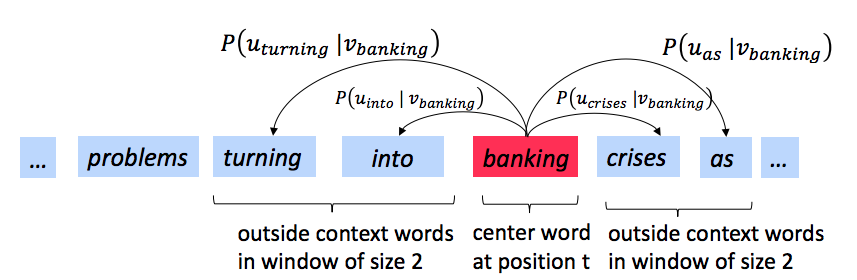
\includegraphics[width=0.6\textwidth]{word2vec.png}
    \caption{The word2vec skip-gram prediction model with window size 2}
    \label{fig:word2vec}
\end{figure}

Skip-gram \texttt{word2vec} aims to learn the probability distribution $P(O|C)$.
Specifically, given a specific word $o$ and a specific word $c$, we want to predict $P(O=o|C=c)$: the probability that word $o$ is an `outside' word for $c$ (i.e., that it falls within the contextual window of $c$).
We model this probability by taking the softmax function over a series of vector dot-products: % I added the word "softmax" here because I bet a lot of students will have forgotten what softmax is and why the loss fn is called naive softmax. but if this is too wordy we can just take it out

\begin{equation}
 P(O=o \mid C=c) = \frac{\exp(\bu_{o}^\top \bv_c)}{\sum_{w \in \text{Vocab}} \exp(\bu_{w}^\top \bv_c)}
 \label{word2vec_condprob}
\end{equation}

For each word, we learn vectors $u$ and $v$, where $\bu_o$ is the `outside' vector representing outside word $o$, and $\bv_c$ is the `center' vector representing center word $c$. 
We store these parameters in two matrices, $\bU$ and $\bV$.
The columns of $\bU$ are all the `outside' vectors $\bu_{w}$;
the columns of $\bV$ are all of the `center' vectors $\bv_{w}$. 
Both $\bU$ and $\bV$ contain a vector for every $w \in \text{Vocabulary}$.\footnote{Assume that every word in our vocabulary is matched to an integer number $k$. Bolded lowercase letters represent vectors. $\bu_{k}$ is both the $k^{th}$ column of $\bU$ and the `outside' word vector for the word indexed by $k$. $\bv_k$ is both the $k^{th}$ column of $\bV$ and the `center' word vector for the word indexed by $k$. \textbf{In order to simplify notation we shall interchangeably use $k$ to refer to word $k$ and the index of word $k$.}}\newline

%We can think of the probability distribution $P(O|C)$ as a prediction function that we can approximate via supervised learning. For any training example, we will have a single $o$ and $c$. We will then compute a value $P(O=o|C=c)$ and report the loss. 
Recall from lectures that, for a single pair of words $c$ and $o$, the loss is given by:

\begin{equation} 
\bJ_{\text{naive-softmax}}(\bv_c, o, \bU) = -\log P(O=o| C=c).
\label{naive-softmax}
\end{equation}

We can view this loss as the cross-entropy\footnote{The \textbf{cross-entropy loss} between the true (discrete) probability distribution $p$ and another distribution $q$ is $-\sum_i p_i \log(q_i)$.} between the true distribution $\by$ and the predicted distribution $\hat{\by}$, for a particular center word c and a particular outside word o. 
Here, both $\by$ and $\hat{\by}$ are vectors with length equal to the number of words in the vocabulary.
Furthermore, the $k^{th}$ entry in these vectors indicates the conditional probability of the $k^{th}$ word being an `outside word' for the given $c$. 
The true empirical distribution $\by$ is a one-hot vector with a 1 for the true outside word $o$, and 0 everywhere else, for this particular example of center word c and outside word o.\footnote{Note that the true conditional probability distribution of context words for the entire training dataset would not be one-hot.}
The predicted distribution $\hat{\by}$ is the probability distribution $P(O|C=c)$ given by our model in equation (\ref{word2vec_condprob}). \newline

\textbf{Note:} Throughout this homework, when computing derivatives, please use the method reviewed during the lecture (i.e. no Taylor Series Approximations).

\clearpage
\begin{parts}
\part[2]
Prove that the naive-softmax loss (Equation \ref{naive-softmax}) is the same as the cross-entropy loss between $\by$  and $\hat{\by}$, i.e. (note that $\by$ 
 (true distribution), $\hat{\by}$ (predicted distribution) are vectors and $\hat{\by}_o$ is a scalar):

\begin{equation} 
-\sum_{w \in \text{Vocab}} \by_w \log(\hat{\by}_w) = - \log (\hat{\by}_o).
\end{equation}

Your answer should be one line. You may describe your answer in words.
transitions

\ifans{

    Given the above conditions, the true empirical distribution $\by$ is a one-hot vector in this particular example of center word c and outside word o. 
    \begin{gather*}
        \by_o=1 \\
        \by_{w'}=0, \ w'\in \text{Vocab}-\{o\}
    \end{gather*}
    So, there are transitions below:
    \begin{align*}
        - \sum_{w \in \text{Vocab}}\by_w \log(\hat{\by}_w) &=-(\by_{w_1} \log(\hat{\by}_{w_1})+\dots+\by_{o} \log(\hat{\by}_{o})+\dots+\by_{w_n} \log(\hat{\by}_{w_n}))\\
        &=-(0 \cdot \log(\hat{\by}_{w_1})+\dots+1 \cdot \log(\hat{\by}_{o})+\dots+0 \cdot \log(\hat{\by}_{w_n}))\\
        &=-\log(\hat{\by}_o)
    \end{align*}
}

% Question 1-B
\part[6]
\begin{enumerate}[label=\roman*.]
    \item 
    Compute the partial derivative of $\bJ_{\text{naive-softmax}}(\bv_c, o, \bU)$ with respect to $\bv_c$. \emph{Please write your answer in terms of $\by$, $\hat{\by}$, $\bU$, and show your work to receive full credit}.
    \begin{itemize} 
        \item \textbf{Note}: Your final answers for the partial derivative should follow the shape convention: the partial derivative of any function $f(x)$ with respect to $x$ should have the \textbf{same shape} as $x$.\footnote{This allows us to efficiently minimize a function using gradient descent without worrying about reshaping or dimension mismatching. While following the shape convention, we're guaranteed that $\theta:= \theta - \alpha\frac{\partial J(\theta)}{\partial \theta}$ is a well-defined update rule.}
        \item Please provide your answers for the partial derivative in vectorized form. For example, when we ask you to write your answers in terms of $\by$, $\hat{\by}$, and $\bU$, you may not refer to specific elements of these terms in your final answer (such as $\by_1$, $\by_2$, $\dots$). 
    \end{itemize}
    \item
    When is the gradient you computed equal to zero? \\
    \textbf{Hint:} You may wish to review and use some introductory linear algebra concepts.
    \item
    The gradient you found is the difference between the two terms. Provide an interpretation of how each of these terms improves the word vector when this gradient is subtracted from the word vector $v_c$.

\end{enumerate}

\ifans{
    \begin{enumerate}[label=\roman*.]
        \item Here is the full transitions:
            \begin{align*}
                \frac{\partial \bJ_{\text{naive-softmax}}(\bv_c,o,\bU)}{\partial \bv_c} &= \frac{\partial}{\partial \bv_c}(-\log P(O=o|C=c))\\
                &=\frac{\partial}{\partial \bv_c}\left(-\log \frac{\exp(\bu_{o}^\top \bv_c)}{\sum_{w \in \text{Vocab}} \exp(\bu_{w}^\top \bv_c)}\right)\\
                &= - \frac{\partial}{\partial \bv_c} \left(\bu_{o}^\top \bv_c - \log \sum_{w \in \text{Vocab}} \exp(\bu_{w}^\top \bv_c)\right)\\
                &=- \frac{\partial \bu_{o}^\top \bv_c}{\partial \bv_c} + \frac{\partial}{\partial \bv_c} \log \sum_{w \in \text{Vocab}} \exp(\bu_{w}^\top \bv_c)\\
                &= - \bu_o^\top + d
            \end{align*}
            where 
            \begin{align*}
                d &= \frac{\partial}{\partial \bv_c} \log \sum_{w \in \text{Vocab}} \exp(\bu_{w}^\top \bv_c)\\
                &= \frac{1}{\sum_{w \in \text{Vocab}} \exp(\bu_{w}^\top \bv_c)} \sum_{w \in \text{Vocab}} \frac{\partial}{\partial \bv_c} \exp(\bu_{w}^\top \bv_c)\\
                &= \frac{1}{\sum_{w \in \text{Vocab}} \exp(\bu_{w}^\top \bv_c)} \sum_{w \in \text{Vocab}} \exp(\bu_{w}^\top \bv_c) \bu_w^\top\\
                &= \sum_{x \in \text{Vocab}} \frac{\exp(\bu_{x}^\top \bv_c) \bu_x^\top}{\sum_{w \in \text{Vocab}} \exp(\bu_{w}^\top \bv_c)}\\
                &=\sum_{x \in \text{Vocab}} P(X=x \mid C=c) \bu_x^\top
            \end{align*}
            so
            \begin{align*}
                \frac{\partial \bJ_{\text{naive-softmax}}(\bv_c,o,\bU)}{\partial \bv_c} &= - \bu_o^\top + \sum_{x \in \text{Vocab}} P(X=x \mid C=c) \bu_x^\top\\
                &= -\bu_o^\top + \sum_{x \in \text{Vocab}} \hat{\by}_x \bu_x^\top\\
                &= \hat{\by}_1 \bu_1^\top + \dots + (\hat{\by}_o - 1) \bu_o^\top + \dots + \hat{\by}_{\|\text{Vocab}\|} \bu_{\|\text{Vocab}\|}^\top
            \end{align*}
            notice that $\by_o=1,\ \by_{w'}=0,\ w' \ne o$:
            \begin{align*}
                \frac{\partial \bJ_{\text{naive-softmax}}(\bv_c,o,\bU)}{\partial \bv_c} &=\left( \begin{bmatrix} \hat{\by}_1 \\ \vdots \\ \hat{\by}_o\\ \vdots \\ \hat{\by}_{\|\text{Vocab}\|}\end{bmatrix} - \begin{bmatrix} \by_1 \\ \vdots \\ \by_o\\ \vdots \\ \by_{\|\text{Vocab}\|}\end{bmatrix} \right)^\top \begin{bmatrix} \bu_1^\top \\ \vdots \\ \bu_o^\top\\ \vdots \\ \bu_{\|\text{Vocab}\|}^\top \end{bmatrix}\\
                &=(\hat{\by} - \by)^\top \bU^\top
            \end{align*}
            since the note mentioned above, the result should have the same shape as $\bv_c$,
            \begin{align*}
                \frac{\partial \bJ_{\text{naive-softmax}}(\bv_c,o,\bU)}{\partial \bv_c} &=\bU (\hat{\by} - \by)
            \end{align*}
        \item The gradient is equal to zero when $(\hat{\by}-\by)$ lies in the null space of the matrix $\bU$ which stores the outside word vectors as columns. For a matrix $\bU \in \R^{d \times |\text{Vocab}|}$, where the embedding dimension $d$ is much smaller than the vocabulary size $|\text{Vocab}|$, the columns are linearly dependent, so there exist solutions with $\hat{\by} \ne \by$.
        \item The gradient descent step can be defined as follows:
            \begin{equation*}
                \bv_c^{\text{new}} \gets \bv_c^{\text{old}} - \eta\bU\hat{\by} +\eta\bU\by 
            \end{equation*}
            , where $\eta$ is the step size. Intuitively speaking, adding the vector $\eta\bU\by$ to $\bv_c^{\text{old}}$ will make $\bv_c$ move towards the direction of $\bu_o$ of the outside word $o$ which lies in the context window of the center word $c$. On the other hand, subtracting the vector $\eta\bU\hat{\by}$ will make $\bv_c$ move away from all the other vectors in $\bU$. Note that all probabilities follow $0<\hat{\by_i}<1$.
    \end{enumerate}
}

% Question 1-C
\part[1]
In many downstream applications using word embeddings, L2 normalized vectors (e.g. $\mathbf{u}/||\mathbf{u}||_2$ where $||\mathbf{u}||_2 = \sqrt{\sum_i u_i^2}$) are used instead of their raw forms (e.g. $\mathbf{u}$). Let’s consider a hypothetical downstream task of binary classification of phrases as being positive or negative, where you decide the sign based on the sum of individual embeddings of the words. When would L2 normalization take away useful information for the downstream task? When would it not?

\textbf{Hint:} Consider the case where $\mathbf{u}_x = \alpha\mathbf{u}_y$ for some words $x \neq y$ and some scalar $\alpha$. When $\alpha$ is positive, what will be the value of normalized  $\mathbf{u}_x$ and normalized $\mathbf{u}_y$? How might $\mathbf{u}_x$ and $\mathbf{u}_y$ be related for such a normalization to affect or not affect the resulting classification?

\ifans{
    In the case where $\mathbf{u}_x = \alpha\mathbf{u}_y$ for some words $x \neq y$ and some scalar $\alpha$, when $\alpha$ is positive, the value of normalized  $\mathbf{u}_x$ and normalized $\mathbf{u}_y$ are same. So L2 normalization take away useful information between $x$ and $y$. On the other hand, when there is no such $\alpha > 0$ that can make $\mathbf{u}_x = \alpha\mathbf{u}_y$, L2 normalization will keep the difference between $x$ and $y$.

    $\downarrow\downarrow\downarrow$maybe a better answer$\downarrow\downarrow\downarrow$

    First of all, word embeddings are vectors fully described by magnitude and direction. Suppose there exists a word embedding $\bv = \alpha \bu$, where $\alpha$ is a scalar. The normalized form of $\bu$ is $\frac{\bu}{\|\bu\|}$ and $\frac{\alpha\bu}{|\alpha|\|\bu\|}$ for $\bv$. As can be observed, the magnitude information of $\bv$ is thrown away after L2 normalization is done. For a task that takes magnitude (e.g., binary classification based on the sum of embeddings) into consideration, L2 normalization will affect the result (e.g., the sum of leading to change of sign).
}

% Question 1-D
\part[5] 
Compute the partial derivatives of $\bJ_{\text{naive-softmax}}(\bv_c, o, \bU)$ with respect to each of the `outside' word vectors, $\bu_w$'s. There will be two cases: when $w=o$, the true `outside' word vector, and $w \neq o$, for all other words. Please write your answer in terms of $\by$, $\hat{\by}$, and $\bv_c$. In this subpart, you may use specific elements within these terms as well (such as $\by_1$, $\by_2$, $\dots$). Note that $\bu_w$ is a vector while $\by_1, \by_2, \dots$ are scalars. Show your work to receive full credit.

\ifans{
    \begin{align*}
        \frac{\partial \bJ_{\text{naive-softmax}}(\bv_c,o,\bU)}{\partial \bu_o} &= \frac{\partial}{\partial \bu_o} \left( - \log \frac{\exp(\bu_o^\top \bv_c)}{\sum_{w \in \text{V}} \exp(\bu_w^\top \bv_c)}\right)\\
        &= \frac{\partial}{\partial \bu_o} \left( - \bu_o^\top \bv_c + \log \sum_{w \in \text{V}} \exp(\bu_w^\top \bv_c)\right)\\
        &= -\bv_c + \frac{1}{\sum_{w \in \text{V}} \exp(\bu_w^\top \bv_c)} \frac{\partial}{\partial \bu_o} \exp(\bu_o^\top \bv_c)\\
        &= -\bv_c + \frac{\exp(\bu_o^\top \bv_c)}{\sum_{w \in \text{V}} \exp(\bu_w^\top \bv_c)} \bv_c\\
        &= (\hat{\by}_o - 1) \bv_c = (\hat{\by}_o - \by_o) \bv_c
    \end{align*}
    \begin{align*}
        \frac{\partial \bJ_{\text{naive-softmax}}(\bv_c,o,\bU)}{\partial \bu_w} &= \frac{\partial}{\partial \bu_w} \left( - \log \frac{\exp(\bu_o^\top \bv_c)}{\sum_{x \in \text{V}} \exp(\bu_x^\top \bv_c)}\right)\\
        &= \frac{\partial}{\partial \bu_w} \left( - \bu_o^\top \bv_c + \log \sum_{x \in \text{V}} \exp(\bu_x^\top \bv_c)\right)\\
        &= \frac{1}{\sum_{x \in \text{V}} \exp(\bu_x^\top \bv_c)} \frac{\partial}{\partial \bu_w} \exp(\bu_w^\top \bv_c)\\
        &= \frac{\exp(\bu_w^\top \bv_c)}{\sum_{x \in \text{V}} \exp(\bu_x^\top \bv_c)} \bv_c\\
        &= \hat{\by}_w \bv_c = (\hat{\by}_w - \by_w) \bv_c
    \end{align*}
}

% Question 1-E
\part[1]
Write down the partial derivative of $\bJ_{\text{naive-softmax}}(\bv_c, o, \bU)$ with respect to $\bU$. Please break down your answer in terms of the column vectors $\frac{\partial \bJ(\bv_c, o, \bU)}{\partial \bu_1}$, $\frac{\partial \bJ(\bv_c, o, \bU)}{\partial \bu_2}$, $\cdots$, $\frac{\partial \bJ(\bv_c, o, \bU)}{\partial \bu_{|\text{Vocab}|}}$. No derivations are necessary, just an answer in the form of a matrix.

\ifans{
    \begin{align*}
        \frac{\partial \bJ_{\text{naive-softmax}}(\bv_c,o,\bU)}{\partial \bU} &= \begin{bmatrix} \frac{\partial \bJ(\bv_c,o,\bU)}{\partial \bu_1} & \cdots & \frac{\partial \bJ(\bv_c,o,\bU)}{\partial \bu_o} & \cdots & \frac{\partial \bJ(\bv_c,o,\bU)}{\partial \bu_{|\text{V}|}}\end{bmatrix}\\
        &= \begin{bmatrix} (\hat{\by}_1 - \by_1) \bv_c & \cdots & (\hat{\by}_o - \by_o) \bv_c & \cdots & (\hat{\by}_{|\text{V}|} - \by_{|\text{V}|}) \bv_c\end{bmatrix}\\
        &= \bv_c \begin{bmatrix} \hat{\by}_1 - \by_1 & \cdots & \hat{\by}_o - \by_o & \cdots & \hat{\by}_{|\text{V}|} - \by_{|\text{V}|} \end{bmatrix}\\
        &=\bv_c(\hat{\by}-\by)^\top
    \end{align*}
}

\end{parts}